% !TeX root=main.tex
\chapter{بررسی نتایج و نتیجه‌گیری‌}
در این فصل به بررسی نتایج رویکرد ارائه شده و مقایسه‌ی آن با سایر روش‌های پیش‌بینی خواهیم پرداخت و در آخر نتیجه‌گیری و جمع‌بندی کلی ارائه خواهیم کرد.
\section{ روش جامع اعتبارسنجی متقابل k برابری
\label{K-fold CV}}
 
روش جامع اعتبارسنجی متقابل k برابری
\LTRfootnote{k-Fold Cross Validation (K-fold CV)}
رویکردی تثبیت شده برای اعتبارسنجی قدرت الگوریتم‌ها در یادگیری ماشین است.  برای نشان دادن این واقعیت که داروهای جدید چه نوع برهم‌کنشی دارند و برای جلوگیری از پیش‌بینی بیش از حد خوش‌بینانه، اعتبارسنجی متقابل باید به‌طور دقیق طراحی شود. برای جفت داروهایی که هیچ  برهم‌کنشی شناخته شده‌ای ندارند، اعتبارسنجی متقابل سعی در پیش‌بینی نوع برهم‌کنشی جدید بین آنها و داروهای دارای برهم‌کنش شناخته شده دارد. تولید نمونه‌های آموزش و آزمایش به شرح زیر است:

کل مجموعه داده‌ها به k قسمت مساوی تقسیم می‌شوند. k-1 قسمت به عنوان مجموعه داده‌های آموزشی استفاده می‌شود و براساس آن مدل ساخته می‌شود و با یک قسمت باقی‌مانده عملیات ارزیابی انجام می‌شود. فرآیند مزبور به تعداد k مرتبه تکرار خواهد شد، به گونه‌ای که از هر کدام از k قسمت تنها یکبار برای ارزیابی استفاده شده و در هر مرتبه یک دقت
\LTRfootnote{Precision}
برای مدل ساخته شده، محاسبه می‌شود. در این روش ارزیابی دقت نهایی دسته‌بند
\LTRfootnote{Classifier}
برابر با میانگین k دقت محاسبه شده خواهد بود. معمول‌ترین مقداری که در متون علمی برای k در نظر گرفته می‌شود برابر با 5 یا 10 می‌باشد. بدیهی است هر چه مقدار k بزرگتر شود، دقت محاسبه شده برای دسته‌بند قابل اعتماد‌تر بوده و دانش حاصل شده جامع‌تر خواهد بود و البته افزایش زمان ارزیابی دسته‌بند نیز افزایش می یابد که مهم‌ترین مشکل محسوب می‌شود. هر تنظیم و هر مجموعه داده، اعتبارسنجی مختص خود را دارد. در این پایان نامه با توجه به نوع مسئله و روش‌های به‌کارگرفته شده، از دو اعتبارسنجی متقابل 10 برابری متفاوت به منظور تقسیم کردن داده‌ها به دو مجموعه ارزیابی و آموزش در نظر گرفته‌شد که عبارتند از:

\textbf{حالت اول: اعتبارسنجی متقابل 10 برابری بدون برهم‌کنش‌های ناشناخته}

در این حالت 90 درصد از برهم‌کنش‌های مثبت و منفی را به‌طور تصادفی
\LTRfootnote{Random}
انتخاب می‌کنیم. برای مجموعه‌ی ارزیابی نیز 10 درصد باقی‌مانده از برهم‌کنش‌های مثبت و منفی در نظر می‌گیریم. 

در روال اعتبارسنجی حالت اول مدل انتخاب شده و بعضی پارامترهای اساسی، همچون تعداد ایپوک، تعیین مقدار شد. شکل
\ref{ModelSelection}
روند آموزش مدل انتخابی را نشان می‌دهد. طبق انتظار صحت مدل روی داده‌های آموزش صعودی اکید است اما برای داده‌های اعتبارسنجی بعد از ایپوک ۵ فراز و فرودهایی دیده می‌شود.

در نمودار تابع خطا، تا پایان ایپوک ۵، با افزایش ایپوک‌ها، مقدار تابع خطای مدل روی داده‌های آموزش و رو‌ی داده‌های اعتبارسنجی کم می‌شود. بعد از ایپوک ۵ روند مدل روی داده‌های آموزشی ادامه می‌یابد اما روند برروی داده‌های اعتبارسنجی برعکس می‌شود. به‌معنای دیگر بیش‌برازش رخ می‌دهد. لذا براساس نمودارها تعداد ایپوک مناسب در این مرحله ۵ درنظر گرفته‌شد.

\begin{figure}[!h]
	%\centering
	\begin{minipage}[b]{0.99\linewidth} 
    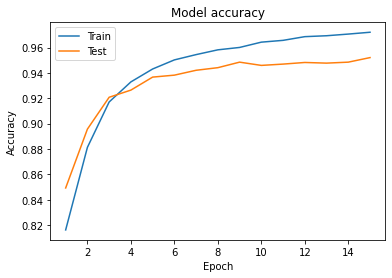
\includegraphics[width=.55\textwidth]{section4/ModelSelection/selectedModelAcc.png} 
    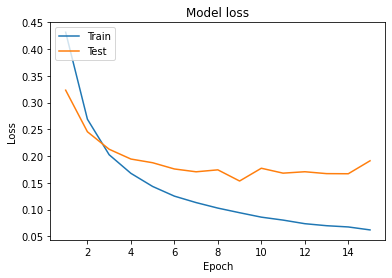
\includegraphics[width=.55\textwidth]{section4/ModelSelection/selectedModelLoss.png} 
\end{minipage}
	\caption{موارد صحت و مقادیر تابع خطا برای شماره ایپوک‌های مختلف}
در شکل راست صحت مدل روی داده‌های آموزش و اعتبارسنجی در طی ۱۵ ایپوک نشان داده می‌شود و در شکل چپ مقادیر تابع خطا در ایپوک‌های مختلف مشاهده می‌شود.
	\label{ModelSelection}
\end{figure}


\textbf{
حالت دوم:اعتبارسنجی متقابل 10 برابری همراه با برهم‌کنش‌های ناشناخته}

در این حالت مجموعه همه برهم‌کنش‌ها (مثبت، منفی، صفرهای مرحله اول) را به 10 دسته مساوی تقسیم می‌کنیم. یک دسته را به‌عنوان مجموعه ارزیابی و 9 دسته دیگر را به‌عنوان مجموعه‌ داده‌ی آموزش درنظر می‌گیریم. همه صفرهای مرحله‌ی قبل را هم به 10 قسمت تقسیم کرده و به نسبت ۱ به ۹ هم به مجموعه‌ی ارزیابی و هم به مجموعه‌ی آموزش اضافه می‌کنیم.

در روال اعتبارسنجی حالت دوم مدل پیشین با کم‌ترین تغییرات برای پیش‌بینی سه‌کلاسه آموزش داده ‌شد. علاوه‌براین، پارامتر اساسی تعداد ایپوک، تعیین مقدار شد. شکل
\ref{lastTripleModel}
روند آموزش را نشان می‌دهد. روند صحت مدل روی داده‌های آموزش با افزایش ایپوک‌ها صعودی اکید است اما برای داده‌های اعتبارسنجی، مدل بعد از ایپوک ۹ مقدار صحت ثابت و کمی افول می‌کند.

در نمودار تابع خطا، تا پایان ایپوک ۹، با افزایش ایپوک‌ها، مقدار تابع خطای مدل روی داده‌های آموزش و رو‌ی داده‌های اعتبارسنجی کم می‌شود. بعد از ایپوک ۹ روند مدل روی داده‌های آموزشی ادامه می‌یابد اما روند برروی داده‌های اعتبارسنجی گاهی بالا و گاهی پایین می‌رود. بدان معناست که احتمال بیش‌برازش بعد از ایپوک ۹ وجود دارد. لذا براساس نمودارها تعداد ایپوک مناسب برای مدل پیش‌بینی سه‌کلاسه ۹ می‌باشد.
\begin{figure}[!h]
%\centering
\begin{minipage}[b]{0.99\linewidth}
    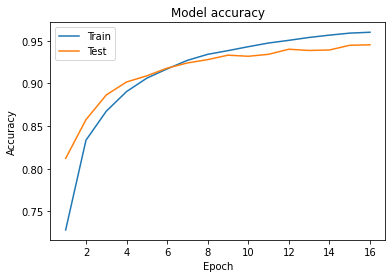
\includegraphics[width=.55\textwidth]{section4/lastTripleModel/modelTripleACC.png}
    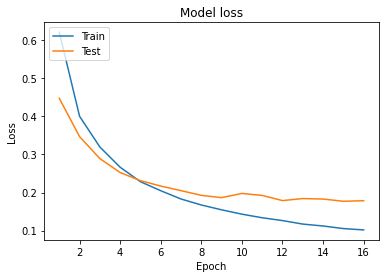
\includegraphics[width=.55\textwidth]{section4/lastTripleModel/modelTripleLoss.png}
\end{minipage}
	\caption{نمودار صحت و مقادیر تابع خطا برای شماره ایپوک‌های مختلف}
در شکل راست صحت مدل روی داده‌های آموزش و اعتبارسنجی در طی ۱۶ ایپوک نشان داده می‌شود و در شکل چپ مقادیر تابع خطا در ایپوک‌های مختلف مشاهده می‌شود.
\label{lastTripleModel}
\end{figure}

\section{معرفی معیارهای سنجش}

به‌ منظور مقایسه عملکرد روش خود با سایر روش‌های موجود، از چهار معیار سنجش، 
$F_{measure}$،
صحت
\LTRfootnote{Accuracy}،
مساحت زیر نمودار منحنی مشخصه‌ی عملکرد سیستم (AUC)
\LTRfootnote{Area Under Roc Curve}
و مساحت زیر نمودار بازخوانی-دقت (AUPR) 
\LTRfootnote{Area Under Precision-Recall Curve}
استفاده شده ‌است. برای تعریف این معیار ها ابتدا چهار معیار شمارشی در این زمینه را در جدول 
\ref{f1}
معرفی کرده‌ایم.
\begin{table}[h!]
\centering 
\begin{tabular}{|c|c|c|c|}
\hline
& پیش‌بینی برهم‌کنش مثبت	& 
پیش‌بینی برهم‌کنش منفی 
\\
\hline
در واقعیت برهم‌کنش مثبت	& مثبت درست& منفی نادرست
\\
\hline
در واقعیت برهم‌کنش منفی& مثبت نادرست & منفی درست
 \\\hline
 \end{tabular}
	\caption{
حالت‌های ممکن نتایج یک یادگیری ماشین 
}
	\label{f1}
\end{table}

با استفاده از آن‌ها چهار معیار سنجش به ترتیب زیر تعریف می‌شوند:

\textbf{صحت:}
نسبت نتایج واقعی (مثبت درست و منفی درست) به تمام موارد مورد بررسی است. 

$$ \mbox{صحت} =  \frac{ \mbox{\rl{تعداد مثبت های درست}} + \mbox{\rl{تعداد منفی های درست}}}
{\mbox{\rl{ تعداد کل نمونه ها}}} $$


همان‌طور که از رابطه بالا مشخص است، حاصل‌جمع تعداد مثبت‌های درست و تعداد منفی‌های درست، نشانگر تعداد نمونه‌هایی است که توسط سیستم به‌درستی تشخیص داده شده‌اند.  مشکل استفاده از معیار صحت، این است که این معیار در زمانی که داده‌ها نامتوازن هستند، معیار مناسبی نیست. زیرا در این حالت، رده‌های را که در بین داده‌ها بیشترین آرا را دارد(رده اکثریت) را به تمام داده‌ها نسبت می‌دهد.

\textbf{$F_{measure}$:}
یک میانگین هارمونیک
\LTRfootnote{Harmonic Average}
میان پارامترهای فراخوانی و دقت می‌باشد و هدف اصلی بیشینه کردن این معیار می‌باشد. 
$F_{measure}$
بر اساس رابطه‌ی زیر محاسبه می‌شود.

$$ F_{measure}  =  \frac{ 2\times( \mbox{\rl{دقت}} + \mbox{\rl{فراخوانی}})}
{\mbox{\rl{ دقت}} + \mbox{\rl{فراخوانی}}} $$

هر کدام از معیارهای فراخوانی
\LTRfootnote{Recall}
و دقت نیز طبق رابطه‌های زیر محاسبه می‌شوند.


$$ \mbox{دقت} =  \frac{\mbox{\rl{تعداد مثبت های درست}}}
{\mbox{\rl{تعداد مثبت های درست}} + \mbox{\rl{تعداد منفی های نادرست}}} $$


$$ \mbox{فراخوانی} =  \frac{ \mbox{\rl{تعداد مثبت های درست}}}
{\mbox{\rl{تعداد مثبت های درست}} + \mbox{\rl{تعداد مثبت های نادرست}}} $$


\textbf{مساحت زیر نمودار بازخوانی-دقت:}
نمودار بازخوانی-دقت یک منحنی دو بعدی است که در آن دقت روی محور عرض‌ها و به‌طور مشابه فراخوانی روی محور طول‌ها رسم می‌شوند. به‌بیان دیگر منحنی دقت-فراخوانی مصالحه نسبی میان دقت و فراخوانی در آستانه‌های متفاوت را نشان می‌دهد. سطح زیر این نمودار یکی از مهم‌ترین معیارهای ارزیابی مدل می‌باشد.
 
\textbf{مساحت زیر نمودار منحنی مشخصه‌ی عملکرد سیستم:}
منحنی‌های مشخصه‌ی عملکرد سیستم، منحنی‌های دو بعدی هستند که در آن‌ها نرخ تشخیص صحیح دسته‌ی مثبت(TPR)
\LTRfootnote{True Positive Rate}
روی محور عرض‌ها و به‌طور مشابه نرخ تشخیص غلط دسته‌ی منفی(FPR)
\LTRfootnote{False Positive Rate }
روی محور طول‌ها رسم می‌شوند. به‌بیان دیگر یک منحنی مشخصه عملکرد سیستم مصالحه نسبی میان سودها و هزینه‌ها را نشان می‌دهد. فرمول‌های  نرخ تشخیص غلط دسته‌ی منفی و نرخ تشخیص صحیح دسته‌ی مثبت که در زیر آورده شده‌است، ماهیت این عناصر را روشن می‌کنند.
 
$$ \mbox{\rl{ نرخ تشخیص صحیح دسته مثبت}} =  \frac{ \mbox{\rl{تعداد مثبت های درست}}}
{\mbox{\rl{تعداد مثبت های درست}} + \mbox{\rl{تعداد منفی های نادرست}}} $$ 

 
$$ \mbox{\rl{ نرخ تشخیص صحیح دسته منفی}} =  \frac{ \mbox{\rl{تعداد مثبت های نادرست}}}
{\mbox{\rl{تعداد مثبت های نادرست}} + \mbox{\rl{تعداد منفی های  درست}}} $$ 


\section{مقایسه‌ی نتایج}
طی روال اعتبارسنجی مبسوط در بخش 
\ref{K-fold CV}
مدل تشخیص نوع برهم‌کنش انتخاب و آموزش داده ‌شد. سپس با تشخیص عدم برهم‌کنش‌های محتمل‌تر مدل سه‌کلاسه نهایی ارائه شد. در ادامه برای بررسی قابلیت اطمینان، استواری و کارایی، مدل
\lr{SNF-CNN}
در روال اعتبارسنجی برروی داده آزموده شد. نتایج
\lr{SNF-CNN}
و سایر روش‌ها که برای مقایسه در نظر گرفته شده‌اند، در این بخش ارائه شده و بررسی می‌شوند. قبل از مقایسه‌ی روش‌های مختلف، نمونه‌ای از نتایج اجرای شبکه‌ی عصبی برای تشخیص نوع برهم‌کنش کاهنده و افزاینده ارائه می‌شود.

\begin{table}[h!]
\centering
\begin{tabular}{|c|c|c|c|c|}
\hline
 
تعداد & $F_{score}$ &فراخوانی & دقت&  
\\
\hline

850 & 0/88 & 0/83 & 0/94 & کاهنده
\\
\hline

3052 & 0/97 & 0/99 & 0/95 & افزاینده
\\
\hline

3902 & 0/95 &  &  & صحت 
\\
\hline
 
3902 & 0/93 & 0/91 & 0/95 & \lr{Macro Avg}
\\
\hline

 3902 & 0/95& 0/95 & 0/95 & \lr{Weighted Avg}
\\
\hline
\end{tabular}
	\caption{
گزارش دسته‌بندی نوع برهم‌کنش}
	\label{classificatonReport}
\end{table}

جدول 
\ref{classificatonReport}
 مثالی از نتایج اجرای مدل است که توانایی مدل از جهت دقت، بازخوانی و 
$F_{score}$
در تشخیص نوع برهم‌کنش‌ها نشان می‌دهد. براساس جدول 
\ref{classificatonReport}
دقت مدل در تشخیص برهم‌کنش افزاینده و کاهنده ۹۵ و ۹۴ درصد است درحالی که فراخوانی به ترتیب ۹۹ و ۸۳ درصد می‌باشد. مقدار 
$F_{measure}$
نیز ۹۷ و ۸۸  درصد می‌باشد که توانایی بالاتر مدل در تشخیص برهم‌کنش‌های افزاینده از تعداد بالاتر این نوع برهم‌کنش‌ها می‌آید. نسبت برهم‌کنش افزاینده به کاهنده تقریبا ۴ به ۱ است. 

\begin{table}[h!]
\centering
\begin{tabular}{|c|c|c|c|c|}
\hline
 
تعداد & $F_{score}$ &فراخوانی & دقت&  
\\
\hline

850 & 0/86 & 0/84 & 0/88 & کاهنده
\\
\hline

3000 & 0/96 & 0/95 & 0/96 & عدم برهم‌کنش
\\
\hline

3052 & 0/96 & 0/97 & 0/95 & افزاینده
\\
\hline

6902 & 0/95 &  &  & صحت 
\\
\hline
 
6902 & 0/93 & 0/92 & 0/93 & \lr{Macro Avg}
\\
\hline

 6902 & 0/95& 0/95 & 0/95 & \lr{Weighted Avg}
\\
\hline
\end{tabular}
	\caption{
گزارش دسته‌بندی حالت سه‌کلاسه برهم‌کنش}
	\label{TripleclassificatonReport}
\end{table}
همچنین در جدول 
\ref{TripleclassificatonReport}
گزارش دسته‌بندی برای حالت سه‌کلاسه نشان داده می‌شود. در این اجرا دقت مدل برای تشخیص برهم‌کنش افزاینده، بدون برهم‌کنش و برهم‌کنش کاهنده به ترتیب ۹۵، ۹۶ و ۸۸ درصد است. فراخوانی به ترتیب ۹۷، ۹۵ و ۸۴ درصد است و در نهایت 
$F_{measure}$
۹۶، ۹۶ و ۸۶ درصد می‌باشد. مشاهده شد، توان مدل در حالت سه‌کلاسه مقدار کمی نسبت به دوکلاسه کاهش می‌یابد که می‌تواند دو دلیل داشته ‌باشد.

۱) مسئله سه‌کلاسه از دوکلاسه سخت‌تر است.

۲) صفرها یا عدم برهم‌کنش‌ها لزوما واقعی نبوده و از نظر داروشناسی تایید شده نیستند پس احتمال وجود مقداری اختلال می‌رود.

لذا به دلایل فوق الذکر مقداری کاهش توان مدل در تشخیص سه‌کلاسه دور از انتظار نبود.

از آنجا که الگوریتم‌های پیشین در پیش‌بینی سه‌تایی برهم‌کنش دارو-دارو از 
\lr{AUC}
و 
\lr{AUPR}
بهره می‌برند، لذا نتایج الگوریتم ارائه ‌شده براساس این دو معیار و برای تشخیص برهم‌کنش افزاینده، عدم برهم‌کنش و برهم‌کنش کاهنده مطابق جدول 
\ref{SNF-CNNresult}
می‌باشد. همچنین در جدول برای الگوریتم ارائه ‌شده این تحقیق بازه‌ی بالا و پایین با اطمینان ۹۵ درصد گزارش شده‌است که نشان می‌دهد، نتایج الگوریتم در روال اعتبارسنجی ۱۰تایی تغییرات کمی داشته و الگوریتم ارائه‌شده استوار بوده و قابل اعتماد می‌باشد.

\begin{table}[h!]
\centering 
\begin{tabular}{|c|c|c|c|}
\hline
& AUC	 & AUPR
\\
\hline
افزاینده	& $0/9747 \pm 0/0033$ & $0/9666 \pm 0/0045$
\\
\hline
کاهنده  & $0/9686 \pm 0/0028$ & $0/8221 \pm 0/0184$
\\
\hline
عدم برهم‌کنش & $0/9714 \pm 0/0040$ & $0/9480 \pm 0/0083$
\\\hline
 \end{tabular}
	\caption{
نتایج الگوریتم
\lr{SNF-CNN}
 در پیش‌بینی سه‌کلاسه براساس معیارهای 
\lr{AUC}
و 
\lr{AUPR}
و بازه‌ی اطمینان آن‌ها
}
	\label{SNF-CNNresult}
\end{table}


در جدول 
\ref{AUCAUPR}
نتایج الگوریتم
\lr{SNF-CNN}
برای سه حالت میانگین گرفته ‌شده و در جدول با دیگر الگوریتم‌های سه‌کلاسه موجود مقایسه ‌شده ‌است. طبق جدول 
\ref{AUCAUPR}
الگوریتم ارائه ‌شده اختلاف بالایی نسبت به دیگر الگوریتم‌های برتر مسئله‌ی سه‌تایی، داشته و توانسته الگوریتم‌های دیگر را به چالش بکشد.

\begin{table}[h!]
\centering 
\begin{tabular}{|c|c|c|c|}
\hline
& AUC	& AUPR 
\\
\hline
SNF-CNN	& 0/971 & 0/912
\\
\hline
\rl{\cite{Shi J2019}} BRSNMF & 0/645 & 0/346
\\
\hline
\rl{\cite{Yu H2018}} Semi-NMF & 0/796 & 0/579
\\
\hline
\rl{\cite{Shi J-Y2018}} TMFUF  & 0/842  & 0/526
 \\\hline
 \end{tabular}
	\caption{
مقایسه‌نتایج الگوریتم‌های پیش‌بینی سه‌کلاسه براساس معیارهای 
\lr{AUC}
و 
\lr{AUPR}
}
	\label{AUCAUPR}
\end{table}



\section{نتیجه‌گیری و جمع‌بندی}
در این رساله، با مدل‌سازی مسئله‌ی پیش‌بینی برهم‌کنش دارو-دارو و بهره‌گیری از رویکردهای مسئله‌ی سیستم‌های توصیه‌گر، روشی نوین با نتایج به مراتب بهتر نسبت به کارهای گذشته ارائه دادیم. با بررسی چهار معیار سنجش، صحت، مساحت زیر نمودار منحنی مشخصه‌ی عملکرد سیستم، مساحت زیر نمودار فراخوانی-دقت و 
$F_{measure}$
 دیدیم که روش ما نتایج دقیق‌تری نسبت به سایر روش‌های موجود ارائه می‌کند. همچنین برای بررسی میزان قدرت روش
\lr{SNF-CNN}
در شناسایی برهم‌کنش‌های ناشناخته، تعدادی از برهم‌کنش‌های جدید که مدل آنها را پیش‌بینی کرده است را مورد تحقیق قرار داده‌ایم.





